\chapter{Overall Description}

\section{Product perspective}

The system will be developed from scratch and it will completely replace the legacy system.
\subsection{Class diagram}
The class diagram in \clupautoref{fig:class_diagram} is a high-level representation of the system as a whole.

\begin{figure}[H]
	\centering
	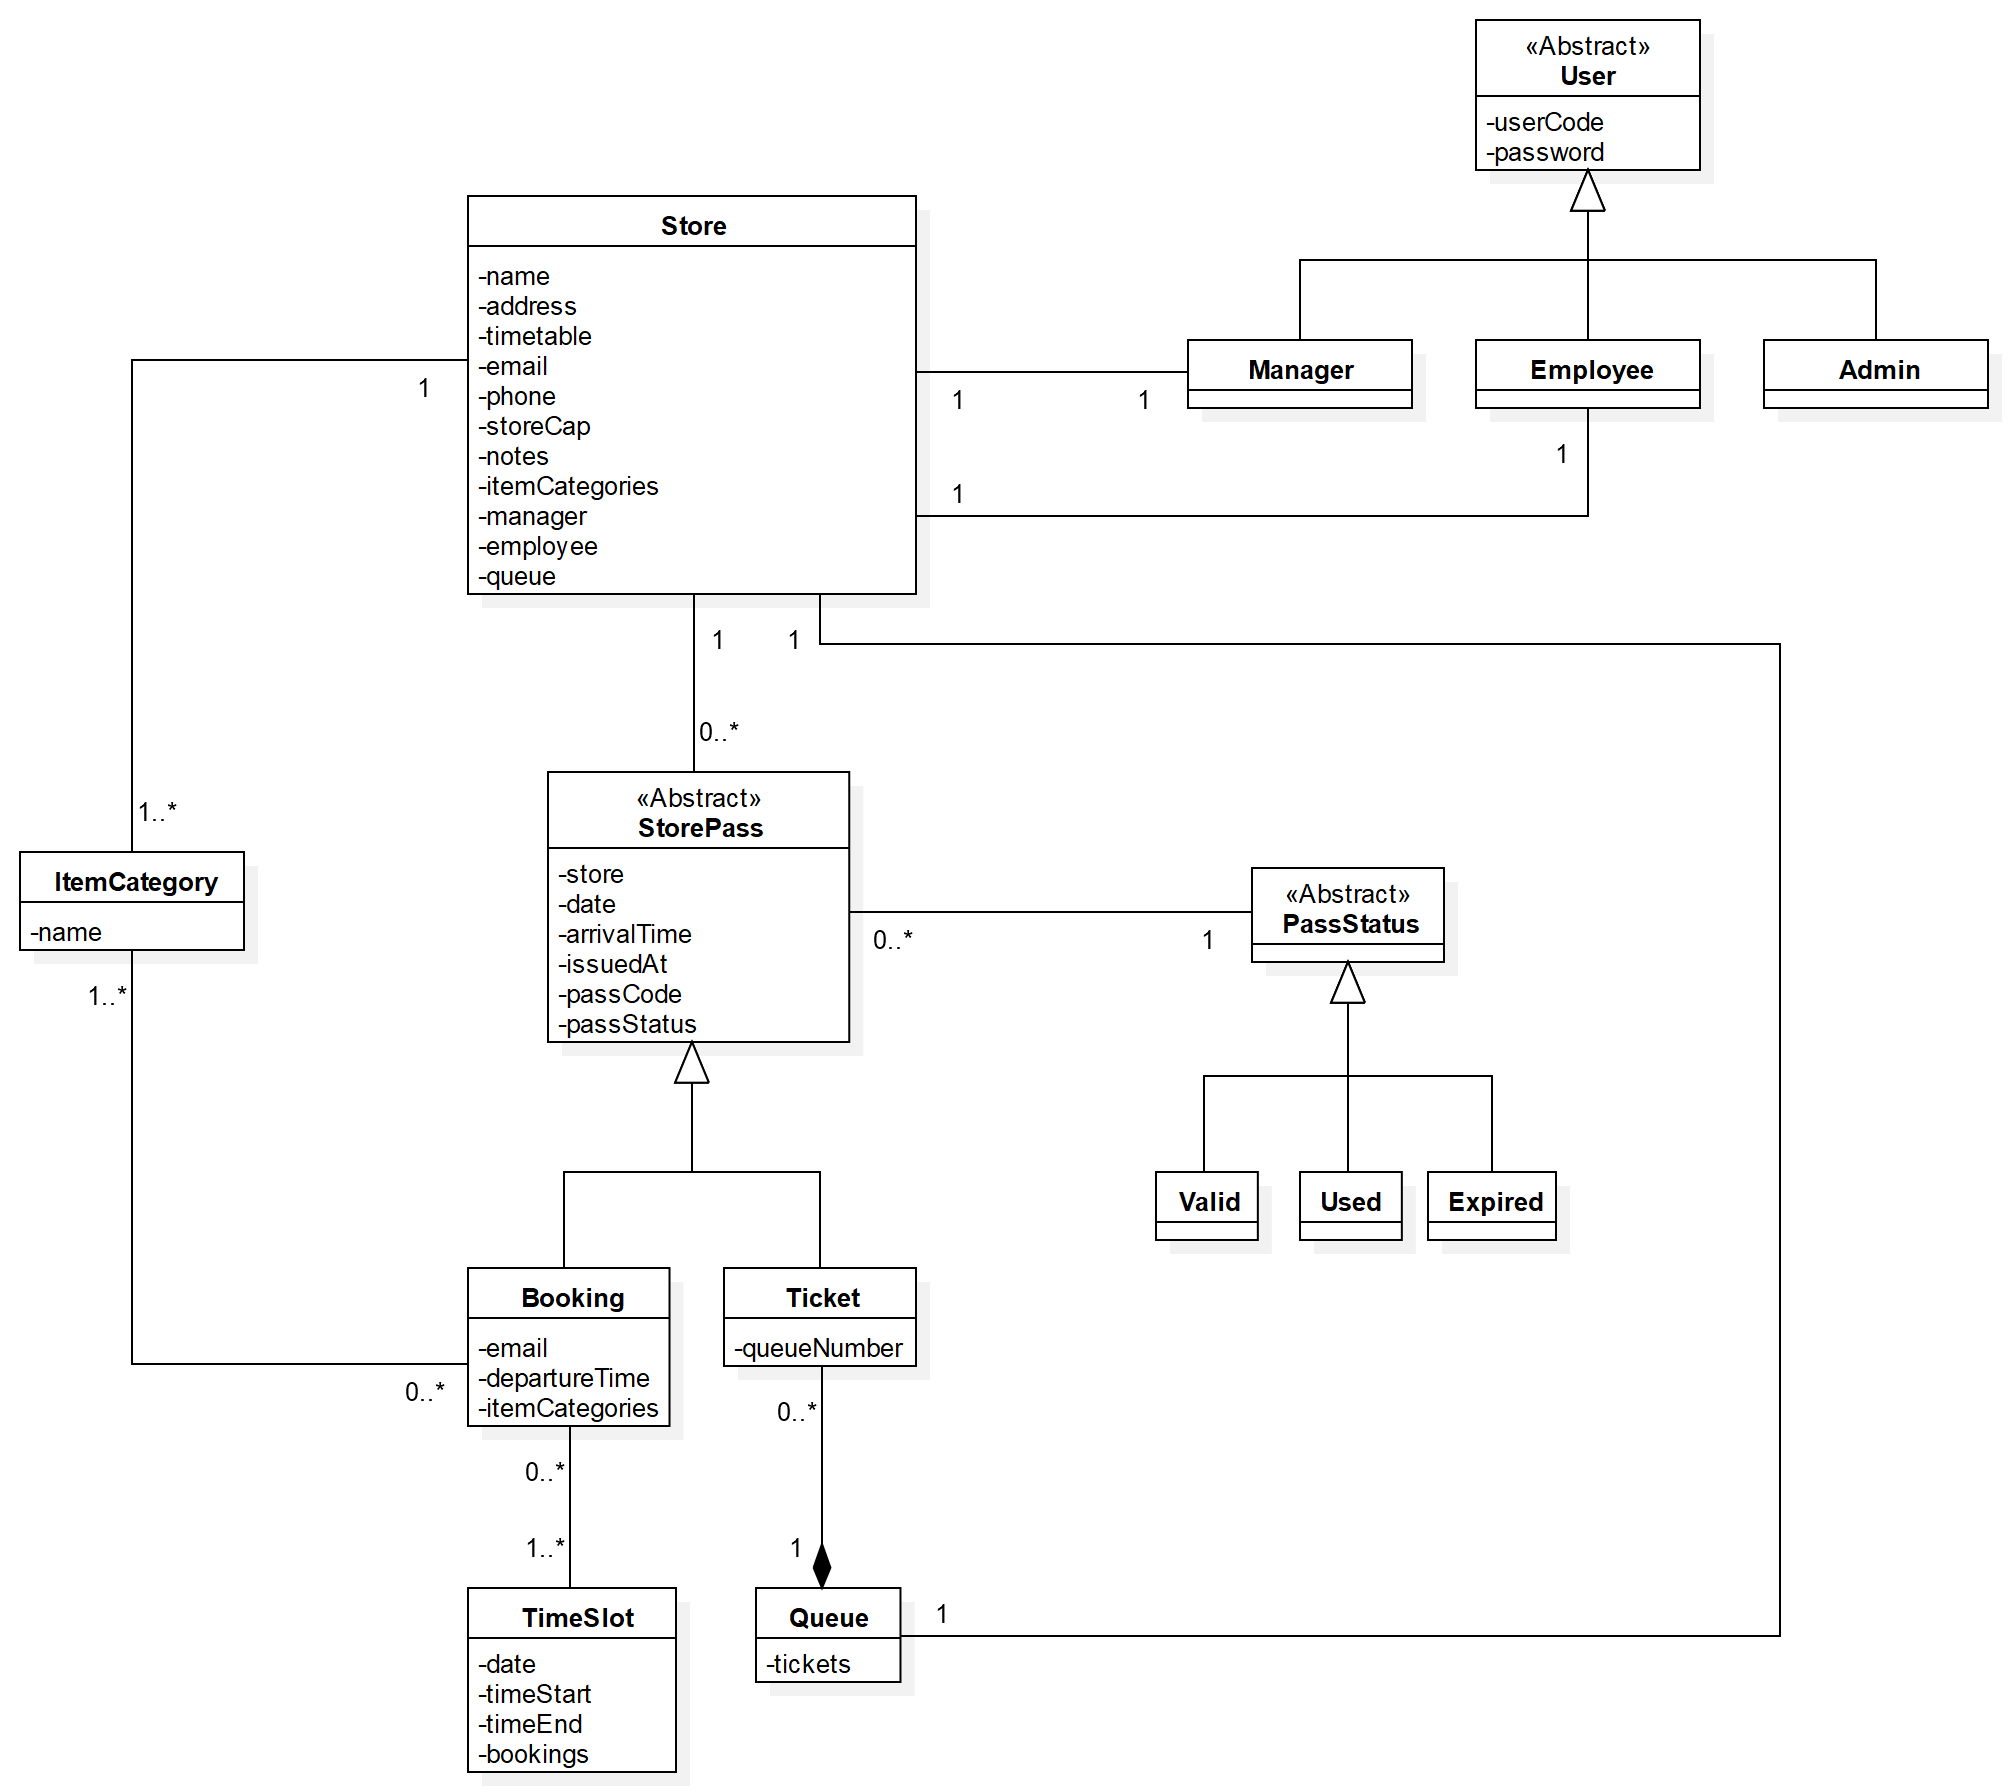
\includegraphics[width=\linewidth]{class_diagram}
	\caption{Class diagram.}
	\label{fig:class_diagram}
\end{figure}


\subsection{State diagrams}
State diagrams describe the behaviour of the system while considering all possible states the objects can have when an event occurs. This analysis helps to clarify the most critical aspects of the system.

\begin{figure}[H]
	\centering
	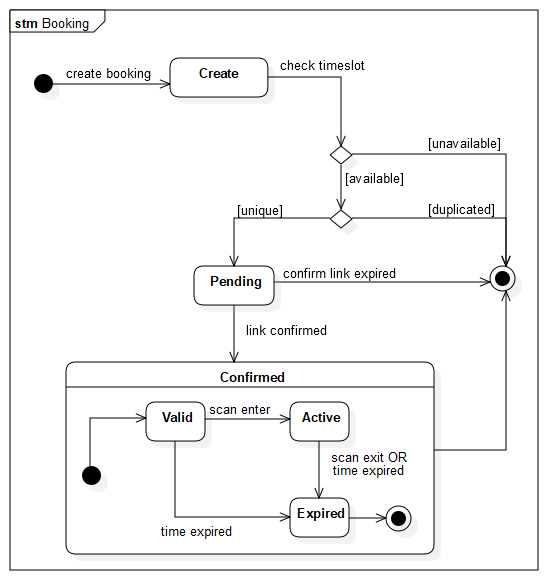
\includegraphics[width=\linewidth]{stm_booking}
	\caption{State diagram: Booking.}
\end{figure}

\begin{figure}[H]
	\centering
	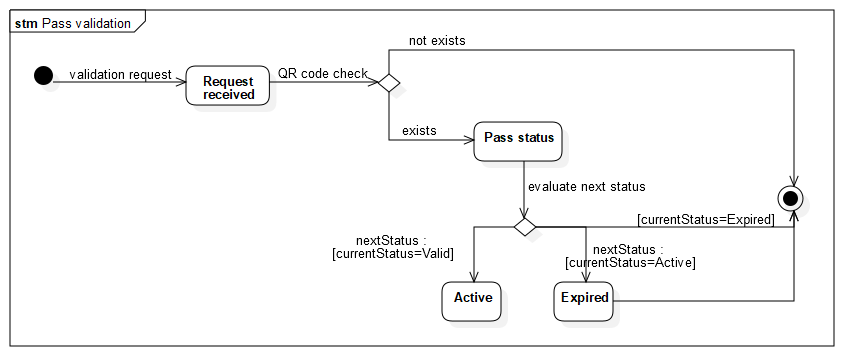
\includegraphics[width=\linewidth]{stm_pass_validation}
	\caption{State diagram: Pass validation.}
\end{figure}


\section{Product functions}\label{desc:prodFunc}
This section provides a summary of the major functions that the software will perform w.r.t. the goals already described in section \clupref{intro:goals}.

\subsection{Store pass function}
	A Store pass, among other things, consists of a QR code and a pass status. The latter identifies the current status inside the pass life-cycle:
	\begin{itemize}
		\item VALID: pass generated but not used yet.
		\item ACTIVE: pass in use.
		\item EXPIRED: pass no longer acceptable. The period of time for which it could be used has ended or the pass has been successfully used.
	\end{itemize}

	The system also takes care of managing delays of customers: a delay greater than 15 minutes will result in the expiration of the pass. This implies that the customer will not be able to enter the store with that pass, instead they shall create a new one.\newline

	Note that to benefit from these functions, the GPS service on customers' smartphones must be enabled, otherwise the application will not work.

	\subsubsection{Queue function}
	The main function of \textit{CLup} is to manage queues. A user who wants to do grocery-shopping will join the queue for a specific store through the system.\newline

	Firstly, the user will be asked to select the store in which he desires to line-up.\newline
	Then the system will prompt the current size of the queue and an estimate of waiting time. If the user is satisfied with his choice it can subscribe to the queue upon completing a CAPTCHA. The operation will be confirmed by the emission of a ticket. The ticket comprehends a queue number, which identify user's position in the queue, and a QR code, which is used for the ticket validation.

	At any time the user will be able to check his position in the queue and the \textit{leave-at-time} (i.e. the time they need to depart from their current position to reach the store). When the user has to leave from where he is, the system sends a notification. The current position will be retrieved by the GPS of the user device.

	\subsubsection{Reserve function}
	This advanced function allows customers to "book a visit" to the store.
	A booking has an additional status attribute (i.e. booking status) which can be:
	\begin{itemize}
		\item PENDING: the booking has not been confirmed via email yet.
		\item CONFIRMED: the booking has been confirmed via email.
	\end{itemize}

	Customers are asked to select the store they want to visit. Then they need to fill in a form by indicating:
	\begin{itemize}
		\item an \textbf{email address}, which will be needed to send a receipt and memo to the user;
		\item the \textbf{date} of the visit;
		\item the approximate \textbf{expected duration} of the trip;
	 	\item the main \textbf{categories of items} they intend to buy;
	    \item a \textbf{time slot} chosen from the ones suggested by the system.
	\end{itemize}
	Every field of the form is mandatory, this means that the user must complete all of them, including the solution of a CAPTCHA, in order to submit the reservation.

	Customers will have to make reservations at least one day in advance.\newline
	The system will send an email with a confirmation link to the email address provided. To complete the booking process, the user must click the confirmation link within 24 hours from the time of subscription and in any case at least 1 hour before the chosen time slot. Users who fail to do so will have their booking expired.
	
	Among the available store seats, about the 15\% of them are reserved only for the bookings.\newline
	The time slots will be suggested according to the saturation of the grocery shelves.\newline
	The system will try to balance the number of people in each section of the store. In case of a particularly crowded shelve, the system will disable the booking for that time slot.
	
	Customers are also allowed to delete their booking at any time by going to the right section or by clicking the link sent via email after the reservation.
	Also this function support the \textit{leave-at-time} features, as described above in the Queue Function.

	In addition, for long-term customers, the app suggests a time inferred by the system based on an analysis of the previous visits.

\subsection{Validation function}
The system provides an interface that allows to scan QR codes by using the smartphone camera. This process is required in order to validate store passes.\newline
Ticket validation allows to speed up the check-in process and to increase the number of people in the store. At the same time it helps staff to detect the authenticity of tickets brought to them.\newline
The scan of the QR code will be executed:
\begin{itemize}
	\item at the \textbf{entrance} by a dedicated store employee to control the influx at the store entrance.
	\item at the \textbf{exit} by the cashiers in order to notify the exit of customers from the store. In case any customer loses the QR code inside the store, the cashiers will use a backup QR code.
\end{itemize}

\subsection{Monitor function}
\textit{Customers Line-up} platform grants supermarkets a way to manage queues and customers inside their stores. In particular, \textbf{upon authentication}, it offers three level of access: \textit{manager-level} and \textit{staff-level} for supermarkets and \textit{admin-level} for CLup administrators.

\begin{itemize}
	\item \textbf{Manager level}\newline
	With the \textbf{dashboard UI}, store managers have access to tables and data visualizations of their customers visits and behaviours. In particular, they can monitor the number of people in the queue and the ones inside the store. Then, based on those data they can setup the maximum cap of people inside the store.\newline
	Store managers can view, edit and delete the list of reservations made by the customer.\newline
	Last but not least, they can inspect information about the booked visits at any given time.

	\item \textbf{Entrance-staff level}\newline
	A store employee is able to view data about the number of people in the queue and inside the building. This is needed during the validation of tickets when the check-in staff scans QR and allows customers inside the store.

    \item \textbf{Admin level}\newline
    An administrator of CLup is able to register new supermarkets and generate the respective credentials to access \textit{manager-level} and \textit{staff-level}.
\end{itemize}

	\clearpage


\subsection{Scenarios}

\subsubsection{Scenario 1}\label{sc:first}
John has to go to the supermarket to buy some groceries. Since there is a pandemic going on, he would like to go there as safely as possible.\newline
So he opens CLup, chooses his trusted supermarket and takes a queue ticket. The application tells him to go to the supermarket at 12:30 and since John is about ten minutes away from the store it notifies him to leave at 12:20. Once in the store an employee checks the ticket by scanning his QR code and John can enter the supermarket.
At the exit the cashier will scan again the QR to notify the exit of a customer from the store.

\subsubsection{Scenario 2}\label{sc:second}
Tomorrow John is going to go for work near the largest Essecorta in the province. There is no better opportunity to go shopping in his favourite supermarket.\newline
However, since he will be tight on time, he needs to book a visit to the store so he won't lose even a minute. Thus, he takes his phone and opens CLup, he chooses the store from the list and enters some informations, like the category of items he would like to buy. He adds the desired time slot and finally opens the email that just arrived and confirms his booking: he is now ready to go.

\subsubsection{Scenario 3}\label{sc:third}
John's business appointment near the famous Essecorta has been cancelled. For this reason, he can no longer go to the store.\newline
Since John is a model citizen, he decides to delete the booking that he did with CLup. So he opens the app, he goes to the store pass section and deletes the bookings.

\subsubsection{Scenario 4}\label{sc:fourth}
The CLup admin Bob was contacted from the manager of Superal store near the Cathedral to provide CLup to his customers. After asking him some informations about the store, like Name and PEC, the admin fills the form to register a new store. From now on the customers of Superal can enjoy the service.

\subsubsection{Scenario 5}\label{sc:fifth}
The Superal store has recently expanded due to some renovation works. The manager Alice wants to increase the number of maximum customer inside the store and monitor them.\newline
For doing so, she logs into the system and increases the maximum cap. From that page she also watches the number of customers inside the store.

\clearpage
\subsection{Use cases description}
Use cases capture functional requirements of a system from the users' perspective.

\begin{table}[H]
    \centering
    \begin{tabular}{@{}p{0.25\linewidth}p{0.71\linewidth}@{}}
        \toprule
        \textbf{Name} & Retrieve ticket \\

        \midrule
        \textbf{ID} & \usecaseindex{uc:retrieveTicket} ~\\
        \midrule
        \textbf{Actors} & Customer \\
        \midrule
        \textbf{Entry conditions} &
        \begin{itemize}[leftmargin=.4cm,noitemsep,topsep=0pt,before=\vspace{-3mm},after=\vspace{-4mm}]
            \item The customer has access to the application on their device;
            \item The application is running.
        \end{itemize} \\
        \midrule
        \textbf{Flow of events} &
        \begin{enumerate}[label=\roman*.,leftmargin=.5cm,noitemsep,topsep=0pt,before=\vspace{-3mm},after=\vspace{-4mm}]
            \item The customer selects a store from the home page;
            \item The customer presses the "Retrieve Ticket" button.
            \item The application notifies the customer when it's time to leave.
        \end{enumerate} \\
        \midrule
        \textbf{Exit conditions} & The customer has retrieved a ticket for the selected store. \\
        \midrule
        \textbf{Exceptions} &
        \begin{itemize}[leftmargin=.4cm,noitemsep,topsep=0pt,before=\vspace{-3mm},after=\vspace{-4mm}]
            \item If the customer has already retrieved a ticket for a store, the system displays an error message telling the customer they cannot get more than one ticket simultaneously.
            \item If the system fails to retrieve the GPS location, no notification will be shown.
        \end{itemize} \\
        \bottomrule
    \end{tabular}
    \caption{\textit{Retrieve ticket} use case description.}
\end{table}

\begin{figure}[H]
    \centering
    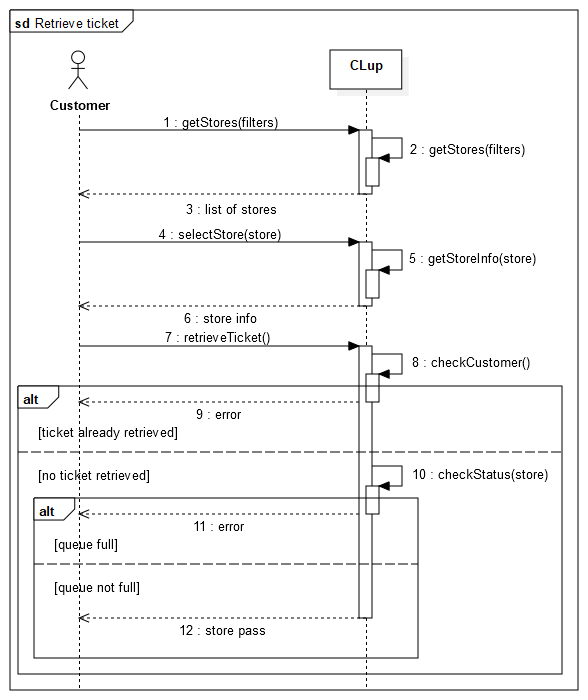
\includegraphics[width=\linewidth]{sd_retrieve_ticket}
    \caption{\textit{Retrieve ticket} sequence diagram.}
\end{figure}

\begin{table}[H]
    \centering
    \begin{tabular}{@{}p{0.25\linewidth}p{0.71\linewidth}@{}}
        \toprule
        \textbf{Name} & Book a visit \\

        \midrule
        \textbf{ID} & \usecaseindex{uc:bookVisit} ~\\
        \midrule
        \textbf{Actors} & Customer \\
        \midrule
        \textbf{Entry conditions} &
        \begin{itemize}[leftmargin=.4cm,noitemsep,topsep=0pt,before=\vspace{-3mm},after=\vspace{-4mm}]
            \item The customer has installed the application on their device;
            \item The application is running.
        \end{itemize} \\
        \midrule
        \textbf{Flow of events} &
        \begin{enumerate}[label=\roman*.,leftmargin=.5cm,noitemsep,topsep=0pt,before=\vspace{-3mm},after=\vspace{-4mm}]
            \item The customer selects a store from the home page;
            \item The customer presses the "Book a visit" button;
            \item The customer inserts their email address, the date, the approximate duration of the visit and the main categories of items they intend to buy;
            \item The customer selects the time slot;
            \item The customer submits the form;
            \item The system shows to the customer the booked visit.
            \item The application notifies the customer when it's time to leave.
        \end{enumerate} \\
        \midrule
        \textbf{Exit conditions} & The customer has retrieved a ticket for the selected store. \\
        \midrule
        \textbf{Exceptions} &
        \begin{itemize}[leftmargin=.4cm,noitemsep,topsep=0pt,before=\vspace{-3mm},after=\vspace{-4mm}]
            \item If the customer has already booked a visit to a store in a certain date, the system displays an error message telling the customer it cannot book again for the same day at the same store;
            \item If the customer selects a date so that there are no more available time slots, the system displays an error message telling the customer to select a different date.
            \item If the system fails to retrieve the GPS location, no notification will be shown.
        \end{itemize} \\

        \bottomrule
    \end{tabular}
    \caption{\textit{Book a visit} use case description.}
\end{table}

\begin{figure}[H]
    \centering
    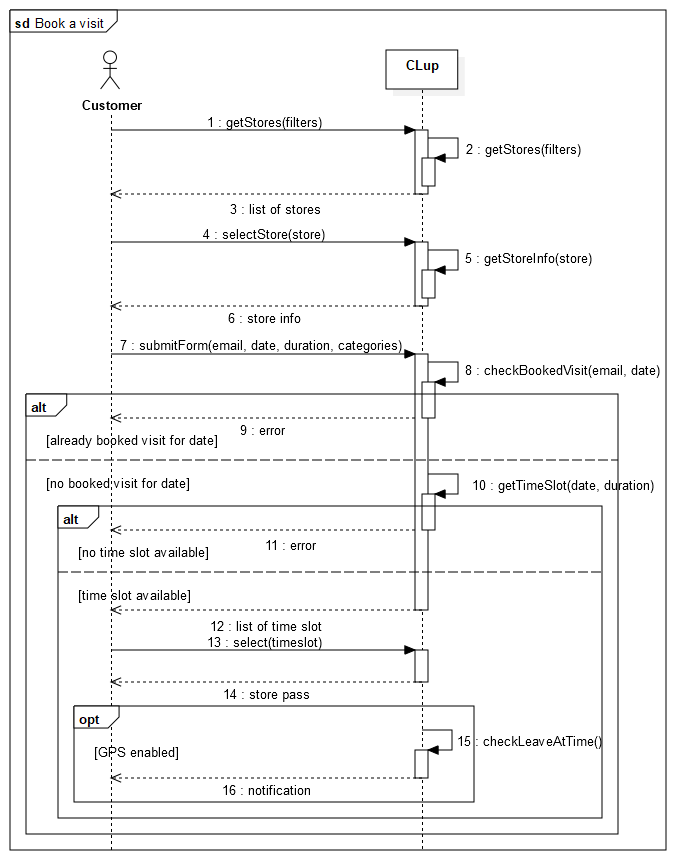
\includegraphics[width=\linewidth]{sd_book_a_visit}
    \caption{\textit{Book a visit} sequence diagram.}
\end{figure}

\begin{table}[H]
    \centering
    \begin{tabular}{@{}p{0.25\linewidth}p{0.71\linewidth}@{}}
        \toprule
        \textbf{Name} & Delete a store pass \\

        \midrule
        \textbf{ID} & \usecaseindex{uc:deletePass} ~\\
        \midrule
        \textbf{Actors} & Customer \\
        \midrule
        \textbf{Entry conditions} &
        \begin{itemize}[leftmargin=.4cm,noitemsep,topsep=0pt,before=\vspace{-3mm},after=\vspace{-4mm}]
            \item The customer has installed the application on their device;
            \item The application is running.
        \end{itemize} \\
        \midrule
        \textbf{Flow of events} &
        \begin{enumerate}[label=\roman*.,leftmargin=.5cm,noitemsep,topsep=0pt,before=\vspace{-3mm},after=\vspace{-4mm}]
            \item The customer swipes to the "My Store Pass" page;
            \item The customer selects one of the available store passes;
            \item The customer presses the "Delete Store Pass" button;
            \item The customer selects "Yes" on the confirmation message;
            \item The customer is notified by the system that the store pass has been deleted successfully.
        \end{enumerate} \\
        \midrule
        \textbf{Exit conditions} & The customer has deleted successfully a store pass. \\
        \midrule
        \textbf{Exceptions} & If the customer has no store pass, the system displays a label: "No store pass available". \\
        \bottomrule
    \end{tabular}
    \caption{\textit{Delete a store pass} use case description.}
\end{table}

\begin{figure}[H]
    \centering
    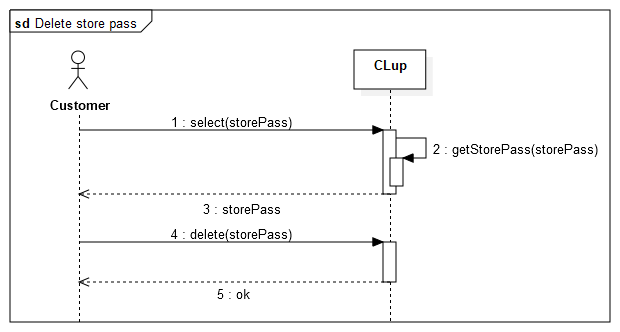
\includegraphics[width=\linewidth]{sd_delete_store_pass}
    \caption{\textit{Delete a store pass} sequence diagram.}
\end{figure}


\begin{table}[H]
    \centering
    \begin{tabular}{@{}p{0.25\linewidth}p{0.71\linewidth}@{}}
        \toprule
        \textbf{Name} & Platform login \\

        \midrule
        \textbf{ID} & \usecaseindex{uc:webLogin} ~\\
        \midrule
        \textbf{Actors} & Store manager, Store employee, CLup admin \\
        \midrule
        \textbf{Entry conditions} &
        \begin{itemize}[leftmargin=.4cm,noitemsep,topsep=0pt,before=\vspace{-3mm},after=\vspace{-4mm}]
            \item The web platform is running.
        \end{itemize} \\
        \midrule
        \textbf{Flow of events} &
        \begin{enumerate}[label=\roman*.,leftmargin=.5cm,noitemsep,topsep=0pt,before=\vspace{-3mm},after=\vspace{-4mm}]
            \item The actor goes to the login page;
            \item The actor inserts their username and password;
            \item The actor submits the form.
        \end{enumerate} \\
        \midrule
        \textbf{Exit conditions} & The actor has successfully logged into the web platform. \\
        \midrule
        \textbf{Exceptions} &
        \begin{itemize}[leftmargin=.4cm,noitemsep,topsep=0pt,before=\vspace{-3mm},after=\vspace{-4mm}]
            \item If the username is not recognized by the system, the credentials are not registered or the username is incorrect. The system notifies the actor and the procedure is aborted.
            \item If the inserted password is wrong, the system notifies the actor and the procedure is aborted.
        \end{itemize} \\

        \bottomrule
    \end{tabular}
    \caption{\textit{Platform login} use case description.}
\end{table}

\begin{figure}[H]
    \centering
    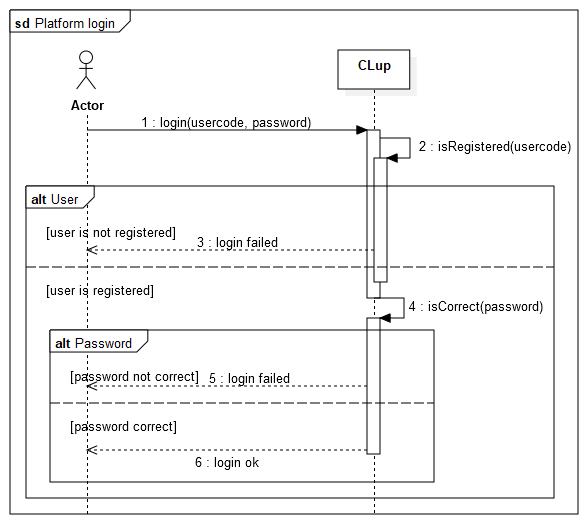
\includegraphics[width=0.8\linewidth]{sd_platform_login}
    \caption{\textit{Platform login} sequence diagram.}
\end{figure}


\begin{table}[H]
    \centering
    \begin{tabular}{@{}p{0.25\linewidth}p{0.71\linewidth}@{}}
        \toprule
        \textbf{Name} & Register new store \\

        \midrule
        \textbf{ID} & \usecaseindex{uc:registerStore} ~\\
        \midrule
        \textbf{Actors} & CLup admin \\
        \midrule
        \textbf{Entry conditions} &
        \begin{itemize}[leftmargin=.4cm,noitemsep,topsep=0pt,before=\vspace{-3mm},after=\vspace{-4mm}]
            \item The platform is running.
            \item The CLup admin is logged in.
            \item The CLup admin has been contacted by a store manager.
        \end{itemize} \\
        \midrule
        \textbf{Flow of events} &
        \begin{enumerate}[label=\roman*.,leftmargin=.5cm,noitemsep,topsep=0pt,before=\vspace{-3mm},after=\vspace{-4mm}]
            \item The CLup admin goes to the "Add supermarket" page;
            \item The CLup admin fills in the form providing store information: name, address, PEC and timetables.
            \item The CLup admin submits the form.
            \item The system generates credentials for the store managers and store employee and send them  via email to the PEC address of the store.
        \end{enumerate} \\
        \midrule
        \textbf{Exit conditions} & The CLup admin has added a store to the platform. \\
        \midrule
        \textbf{Exceptions} &
        \begin{itemize}[leftmargin=.4cm,noitemsep,topsep=0pt,before=\vspace{-3mm},after=\vspace{-4mm}]
            \item If the store name is already used by another store, the system displays an error message asking the CLup admin to insert a different one.
        \end{itemize} \\

        \bottomrule
    \end{tabular}
    \caption{\textit{Register new store} use case description.}
\end{table}

\begin{figure}[H]
    \centering
    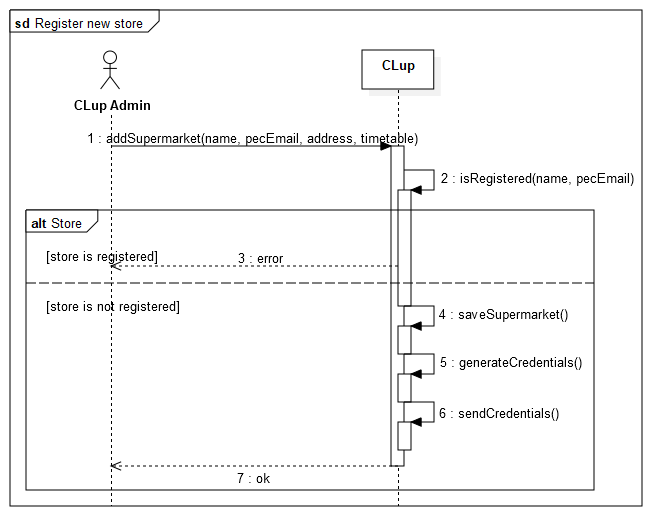
\includegraphics[width=\linewidth]{sd_register_new_store}
    \caption{\textit{Register new store} sequence diagram.}
\end{figure}


\begin{table}[H]
    \centering
    \begin{tabular}{@{}p{0.25\linewidth}p{0.71\linewidth}@{}}
        \toprule
        \textbf{Name} & Monitor bookings \\

        \midrule
        \textbf{ID} & \usecaseindex{uc:monitorBookings} ~\\
        \midrule
        \textbf{Actors} & Store manager \\
        \midrule
        \textbf{Entry conditions} &
        \begin{itemize}[leftmargin=.4cm,noitemsep,topsep=0pt,before=\vspace{-3mm},after=\vspace{-4mm}]
            \item The platform is running.
            \item The store manager is logged in.
        \end{itemize} \\
        \midrule
        \textbf{Flow of events} &
        \begin{enumerate}[label=\roman*.,leftmargin=.5cm,noitemsep,topsep=0pt,before=\vspace{-3mm},after=\vspace{-4mm}]
            \item The Store manager go to the "Manage bookings list" page;
            \item The Store manager can filter bookings by date, time slot and categories;
            \item The system provides to the store manager a list with all the bookings that match the filter. If no filter are provided, a full list of all the bookings is shown.
        \end{enumerate} \\
        \midrule
        \textbf{Exit conditions} & The Store manager view the bookings. \\
        \midrule
        \textbf{Exceptions} &
        \begin{itemize}[leftmargin=.4cm,noitemsep,topsep=0pt,before=\vspace{-3mm},after=\vspace{-4mm}]
            \item If no bookings are available, an error is prompted to the store manager.
        \end{itemize} \\

        \bottomrule
    \end{tabular}
    \caption{\textit{Monitor bookings} use case description.}
\end{table}

\begin{figure}[H]
    \centering
    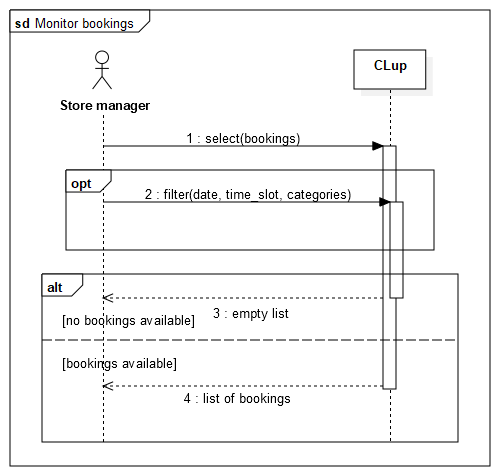
\includegraphics[width=0.7\linewidth]{sd_monitor_bookings}
    \caption{\textit{Monitor bookings} sequence diagram.}
\end{figure}

\begin{table}[H]
    \centering
    \begin{tabular}{@{}p{0.25\linewidth}p{0.71\linewidth}@{}}
        \toprule
        \textbf{Name} & Validate store pass \\

        \midrule
        \textbf{ID} & \usecaseindex{uc:validatePass} ~\\
        \midrule
        \textbf{Actors} & Store employee \\
        \midrule
        \textbf{Entry conditions} &
        \begin{itemize}[leftmargin=.4cm,noitemsep,topsep=0pt,before=\vspace{-3mm},after=\vspace{-4mm}]
            \item The platform is running.
            \item The store employee is logged in.
        \end{itemize} \\
        \midrule
        \textbf{Flow of events} &
        \begin{enumerate}[label=\roman*.,leftmargin=.5cm,noitemsep,topsep=0pt,before=\vspace{-3mm},after=\vspace{-4mm}]
            \item The store employee click on "Scan QR";
            \item The store employee points the camera to the customer's QR code;
            \item The system prompt a response about the validity of the pass;
        \end{enumerate} \\
        \midrule
        \textbf{Exit conditions} & The store pass is accepted. \\
        \midrule
        \textbf{Exceptions} &
        \begin{itemize}[leftmargin=.4cm,noitemsep,topsep=0pt,before=\vspace{-3mm},after=\vspace{-4mm}]
            \item If the store pass is invalid, an error is prompted to the store employee.
        \end{itemize} \\

        \bottomrule
    \end{tabular}
    \caption{\textit{Validate store pass} use case description.}
\end{table}

\begin{figure}[H]
    \centering
    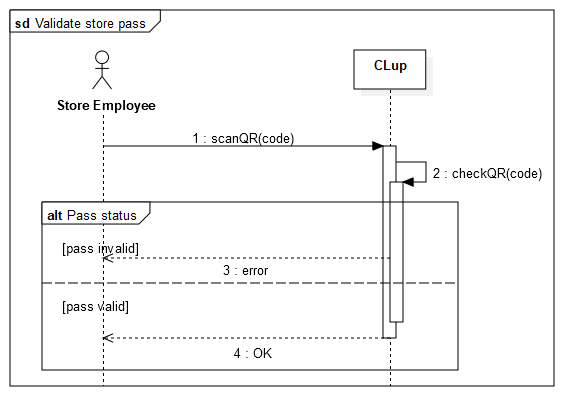
\includegraphics[width=\linewidth]{sd_validate_pass}
    \caption{\textit{Validate store pass} sequence diagram.}
\end{figure}



\section{User characteristics}
CLup has four different groups of users:
\begin{itemize}
	\item \textbf{Customers}: they are customers of the supermarket. They can be of all ages and don't necessarily have experience with technology. They can also be elderly	people who don't have a smartphone at all. For this reason the system should be as easy to use as possible and should provide an alternative way to retrieve a ticket in addition to the mobile app.
	\item \textbf{Store managers}: they are the managers of the store. They manage the number of people who can access the store and can monitor the ones that are in the supermarket. It is reasonable to assume that they have at least a minimum experience with technology and the use of computer. For this reason the dashboard with all the information about customers will be accessible from a web browser.
	\item \textbf{Store employee}: they are the employees of the store. They validate the tickets at the entrance/exit of the store. They could not have experience with technology. For this reason the Store App and the dashboard have a simple interface and the interaction that they should have with them is reduced to the bare minimum.
    \item \textbf{CLup admin}: an operator of CLup able to login to the platform by using his special credentials. It can register supermarkets and generate their credentials. It can also maintain and update the system. Registration for this kind of users is forbidden and it has to be added directly during the system's installation process.
\end{itemize}

\section{Constraints}
In this topic it is put on paper a general description about considerations, boundaries and items that will limit the system's options.

\subsection{Regulatory policies}
The application requests the user's permission in order to retrieve and use their position at runtime.\newline
The email addresses provided when booking through CLup will not be used for commercial purposes or given to third parties.\newline
The email addresses provided by the stores during the registration process must be PEC addresses identified by a Certification Authority.

\subsection{Hardware limitations}
Here is listed where CLup is available depending on the devices. Please note that not all devices are supported.

\begin{itemize}
	\item iPhones with iOS version 13.5 or above, phones and tablets running Android 6 (Marshmallow) or above;
	\item 2G/3G/4G connection or Wi-Fi available;
	\item GPS service;
	\item camera;
	\item modern web browser like Firefox, Chrome or Safari;
	\item internet connection available.
\end{itemize}


\subsection{Interfaces to other applications}
The proper functioning of the app is strictly subordinated to an external map service. This is required to compute travel distance and time for a matrix of origins and destinations (i.e. customer and store position).

A failure in the above described service will translate into the inability to use CLup.

\clearpage

\section{Assumptions and Dependencies}
The properties that hold in the analysed world will be listed below.
\subsection{Domain assumptions}
\begin{enumerate}[label=\textbf{D.\arabic*}]
	\item \itemtext{dom:smartphone}{The majority of the customers has a smartphone with internet available.}
	\item \itemtext{dom:categories}{Customers attains to the declared categories of items.}
	\item \itemtext{dom:internetStores}{Stores have an internet contract.}
	\item \itemtext{dom:pecStores}{Stores have a PEC address.}
	\item \itemtext{dom:workingGps}{GPS modules of customers' smartphones are working properly.}
	\item \itemtext{dom:gpsPrecision}{The precision of the GPS modules of customers' smartphones is greater than twenty meters.}
	\item \itemtext{dom:bringSmartphone}{Customers bring with themselves the smartphone that they used to retrieve a ticket or reserve a time slot.}
    \item \itemtext{dom:oneToOneQr}{A ticket or a booked visit is associated with exactly one person.}
    \item \itemtext{dom:custEmail}{Customers who want to book-a-visit have an email address.}
	\item \itemtext{dom:uniqueName}{Stores have unique names.}
	\item \itemtext{dom:employeeEntrance}{Each store has an employee at the entrance which check-in people.}
	\item \itemtext{dom:empSmartphone}{Store employees have a supplied smartphone with camera.}
	\item \itemtext{dom:empCamera}{The cameras of employees' smartphone are working properly.}
	\item \itemtext{dom:storeRegistered}{Store managers have registered their stores in CLup.}
	\item \itemtext{dom:timeArrival}{Customers comply with the arrival time assigned by the mobile app.}
	\item \itemtext{dom:capStores}{Store managers know the maximum capacity of customers in the building.}
   	\item \itemtext{dom:storeKiosk}{Each store has a Self Service Ticketing Kiosk accessible.}
\end{enumerate}
